%%%%%%%%%%%%%%%%%%%%%%%%%%%%%%%%%%%%%%%%%
% Beamer Presentation
% LaTeX Template
% Version 1.0 (10/11/12)
%
% This template has been downloaded from:
% http://www.LaTeXTemplates.com
%
% License:
% CC BY-NC-SA 3.0 (http://creativecommons.org/licenses/by-nc-sa/3.0/)
%
%%%%%%%%%%%%%%%%%%%%%%%%%%%%%%%%%%%%%%%%%

%----------------------------------------------------------------------------------------
%	PACKAGES AND THEMES
%----------------------------------------------------------------------------------------

\documentclass{beamer}
\usepackage[utf8]{inputenc}
\usepackage[T1]{fontenc}
\usepackage[brazil]{babel}
\usepackage{amsmath}
\usepackage{amsfonts}
\usepackage{amssymb}
\mode<presentation> {

% The Beamer class comes with a number of default slide themes
% which change the colors and layouts of slides. Below this is a list
% of all the themes, uncomment each in turn to see what they look like.

%\usetheme{default}
%\usetheme{AnnArbor}
%\usetheme{Antibes}
%\usetheme{Bergen}
%\usetheme{Berkeley}
%\usetheme{Berlin}
%\usetheme{Boadilla}
\usetheme{CambridgeUS}
%\usetheme{Copenhagen}
%\usetheme{Darmstadt}
%\usetheme{Dresden}
%\usetheme{Frankfurt}
%\usetheme{Goettingen}
%\usetheme{Hannover}
%\usetheme{Ilmenau}
%\usetheme{JuanLesPins}
%\usetheme{Luebeck}
%\usetheme{Madrid}
%\usetheme{Malmoe}
%\usetheme{Marburg}
%\usetheme{Montpellier}
%\usetheme{PaloAlto}
%\usetheme{Pittsburgh}
%\usetheme{Rochester}
%\usetheme{Singapore}
%\usetheme{Szeged}
%\usetheme{Warsaw}

% As well as themes, the Beamer class has a number of color themes
% for any slide theme. Uncomment each of these in turn to see how it
% changes the colors of your current slide theme.

%\usecolortheme{albatross}
%\usecolortheme{beaver}
%\usecolortheme{beetle}
%\usecolortheme{crane}
%\usecolortheme{dolphin}
%\usecolortheme{dove}
%\usecolortheme{fly}
%\usecolortheme{lily}
%\usecolortheme{orchid}
%\usecolortheme{rose}
%\usecolortheme{seagull}
%\usecolortheme{seahorse}
%\usecolortheme{whale}
%\usecolortheme{wolverine}

%\setbeamertemplate{footline} % To remove the footer line in all slides uncomment this line
%\setbeamertemplate{footline}[page number] % To replace the footer line in all slides with a simple slide count uncomment this line

%\setbeamertemplate{navigation symbols}{} % To remove the navigation symbols from the bottom of all slides uncomment this line
}

\usepackage{graphicx} % Allows including images
\usepackage{booktabs} % Allows the use of \toprule, \midrule and \bottomrule in tables

%----------------------------------------------------------------------------------------
%	TITLE PAGE
%----------------------------------------------------------------------------------------

\title[V Workshop de Lx. Comp.]{Primeiros experimentos com o SICK-BR} % The short title appears at the bottom of every slide, the full title is only on the title page

\author{Bruno Ferrari Guide} % Your name
\institute[USP/ Verbio] % Your institution as it will appear on the bottom of every slide, may be shorthand to save space
{Orientador: Marcos Lopes\\
Universidade de São Paulo \\ % Your institution for the title page
\medskip
\textit{bruno.guide@usp.br} % Your email address
}
\date{\today} % Date, can be changed to a custom date

\begin{document}

\begin{frame}
\titlepage % Print the title page as the first slide
\end{frame}

\begin{frame}
\frametitle{Tópicos} % Table of contents slide, comment this block out to remove it
\tableofcontents % Throughout your presentation, if you choose to use \section{} and \subsection{} commands, these will automatically be printed on this slide as an overview of your presentation
\end{frame}

%----------------------------------------------------------------------------------------
%	PRESENTATION SLIDES
%----------------------------------------------------------------------------------------

\section{Introdução}
%------------------------------------------------
	\begin{frame}
\centering \textbf{Introdução\\}
\end{frame}
\begin{frame}
\frametitle{Introdução}
\begin{itemize}
	\item Trabalho desenvolvido majoritariamente com o grupo responsável pela criação do SICK-BR\\
	\item Apresentação 2 em 1:
	\begin{itemize}
		\item Primeiras rodadas de testes com modelos simples diversos usando esse corpus\\
		\item Replicar os testes conduzidos por Fonseca, 2018 em um corpus diferente.\\
	\end{itemize}
	
\end{itemize}
\end{frame}


\section{O Corpus}
%------------------------------------------------
	\begin{frame}
\centering \textbf{O Corpus\\}
\end{frame}

\begin{frame}
\frametitle{SICK-BR}
\begin{figure}
	\centering
	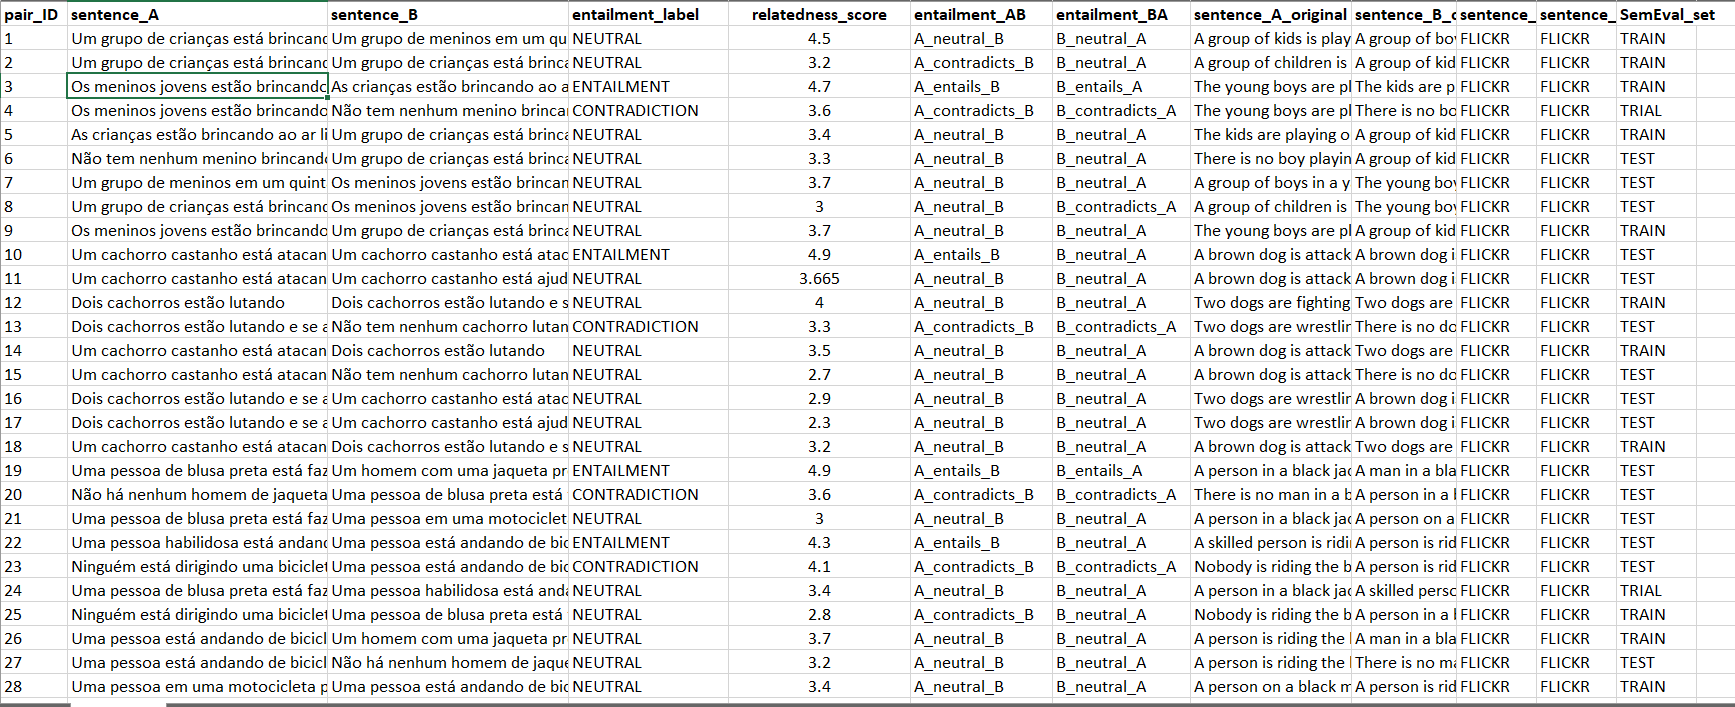
\includegraphics[width=0.7\linewidth]{Sick-BR}
	\caption{Amostra dos dados contidos no SICK-BR}
	\label{fig:sick-br}
\end{figure}

\end{frame}
\section{Baselines}
%------------------------------------------------
	\begin{frame}
\centering \textbf{\textit{Baselines}\\}
\end{frame}

\begin{frame}
	\frametitle{Baseline Majority}
	\begin{itemize}
	\item Esse modelo classifica o par de sentenças de acordo com a classe mais presente no corpus de treinamento.\\	
	\end{itemize}
\end{frame}


\begin{frame}
\frametitle{Baseline Overlap}
\begin{itemize}
	\item Esse modelo extrai dois features do corpus: a quantidade de palavras exclusivas da primeira sentença e a quantidade de palavras exclusivas da segunda.\\
	\item Os features então alimentam uma SVM para fazer a classificação.\\
\end{itemize}
\end{frame}

\section{Naive Bayes}
%------------------------------------------------
	\begin{frame}
\centering \textbf{O classificador Bayesiano Ingênuo (Ou naive bayes)\\}
\end{frame}

\begin{frame}
\frametitle{Bayes}
\begin{figure}
\centering

\includegraphics[width=0.7\linewidth]{bayes-limpo}
\caption{O teorema (ou regra) de Bayes}
\label{fig:bayes-limpo}
\end{figure}

\end{frame}
\begin{frame}
\frametitle{NB - vetor de características}
\begin{itemize}
\item Para atribuir a probabilidade de um par de frases (p) ter como relação uma categoria (c), ou seja, para calcular P(c|p), o modelo trata cada sentença como um vetor de traços ($\bar{p}$).\\
\item Esses traços são as variáveis observadas, caso as palavras daquela sentença e o valor de similaridade entre as duas sentenças.\\
\item Cada valor possível de cada traço tem uma probabilidade relacionada a cada categoria possível.\\
\item Essas probabilidades são extraídas do corpus.\\
\end{itemize}
\end{frame}	


\begin{frame}
\frametitle{NB e SICK-BR: características}
\begin{itemize}
	\item dois grupos de Features foram testados nessa rodada. Um é o Bag-of-Words (BOW) e o outro a similaridade.\\
	\item BOW pois as duas sentenças foram consideradas um saco de palavras, informações sintáticas foram descartadas.\\
	\item No modelo BOW, Cada item do vocabulário (palavras únicas) do corpus de treinamento foi considerado um possível \textit{feature}.\\
	\item As palavras contidas num par de sentenças qualquer entram como features para a classificação daquele par.\\
	
\end{itemize}
\end{frame}

\section{Infernal}
%------------------------------------------------
	\begin{frame}
\centering \textbf{Infernal\footnote{Slides aproveitados de uma apresentação feita por Igor Câmara para o GLiC-USP}\\}
\end{frame}
\begin{frame}[fragile]{INFERNAL}
\begin{itemize}
	\item INFERence in NAtural Language. Desenvolvido na tese de doutorado de Erick Fonseca, defendida em 2018.\\
	\item Sistema de \textbf{engenharia de atributos}.\\
	\item No trabalho do Erick, o corpus utilizado foi o Assin, agora replico no SICK-BR.\\
\end{itemize}
\end{frame}


\begin{frame}[fragile]{INFERNAL: pré-processamento}
\begin{center}
\textbf{Alguns procedimentos de pré-processamento}
\end{center}
\begin{itemize}
\item Anotação de árvores sintáticas.\\
\item Lematização das palavras (um dicionário de lemas + POS Tags para desambiguação)\\
\item Detecção de entidades nomeadas (SpaCy)		\\
\item Alinhamentos lexicais (WordNet e PPDB - \emph{Lexically-Expanded Paraphrase Database})\\
\end{itemize}
\end{frame}


\begin{frame}[fragile]{INFERNAL: atributos}
\begin{center}
\textbf{Atributos}
\end{center}
\begin{itemize}
\item \textbf{BLEU} - métrica usada para avaliação de tradução. Calcula a sobreposição de n-gramas.
\item \textbf{Sobreposição de dependências} - para identificar fenômenos como voz ativa e passiva.
\item \textbf{Nominalização} - identifica a presença de um verbo e um substantivo derivado dele (exemplo: \emph{correr} e \emph{corrida}).
\item \textbf{Proporção e tamanho} - proporção entre quantidade de tokens de ambas as sentenças.
\item \textbf{Argumentos verbais} - correspondência de verbo com sujeito e objeto direto nas duas sentenças. 
\end{itemize}
\end{frame}


\begin{frame}[fragile]{INFERNAL: atributos}
\begin{itemize}
\item \textbf{Negação}: Se um verbo alinhado nas duas sentenças está negado em uma delas.
\item \textbf{Quantidades}: quantidades (iguais ou diferentes) são usadas para se referir a uma palavra alinhada.
\item \textbf{Cosseno das sentenças} - onde o vetor de cada sentença é a média dos vetores de word embedding das palavras que a constituem.
\item \textbf{TED simples}: valor de TED simples, considerando o custo de toda operação como 1. TED normal; normalizado pelo tamanho de cada sentença. 
\end{itemize}
\end{frame}



\begin{frame}[fragile]{INFERNAL: atributos}
\begin{itemize}
\item \textbf{TED com distância de cosseno} - extensão da anterior que calcula custo de substituição como $1-\cos(w_1,w_2)$.
\item \textbf{Sobreposição de palavras} -  Proporção de lemas em comum sobre o total de palavras de $T$ e de $H$.
\item \textbf{Sobreposição de sinônimos} -  Igual ao anterior, mas considerando toda palavra alinhada, não só as com lema idêntico.
\item \textbf{Sobreposição soft} - Idem ao anterior, mas considerando uma medida de similaridade, avaliado pelo cosseno das word embeddings.
\item \textbf{Entidades nomeadas} - identifica entidades nomeadas alinhadas ou desalinhadas nas duas sentenças. 
\end{itemize}
\end{frame}



\section{Resultados}
	\begin{frame}[fragile]
\centering \textbf{Resultados\\}
\end{frame}


\begin{frame}{Resultado - Baselines}
\begin{figure}
	\centering
	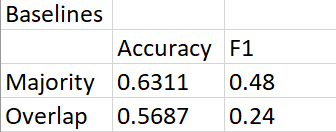
\includegraphics[width=0.7\linewidth]{resultados-baseline}
	\caption{Resultados dos modelos de Baseline no SICK-BR}
	\label{fig:resultados-baseline}
\end{figure}

\end{frame}

\begin{frame}[fragile]{Resultado - Naive Bayes no SICK-BR}
	\begin{figure}
		\centering
		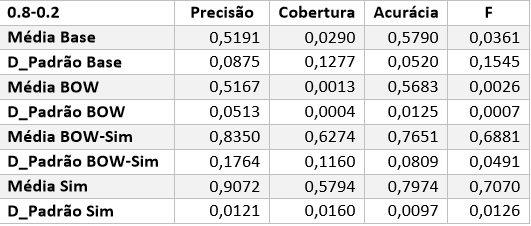
\includegraphics[width=0.7\linewidth]{nb-sickbr}
		\caption{Resultados das versões de Naive Bayes desenvolvidas como primeiro teste no corpus SICK-BR}
		\label{fig:nb-sickbr}
	\end{figure}
	
\end{frame}

\begin{frame}[fragile]{Resultado - Infernal no Assin}
\begin{figure}
	\centering
	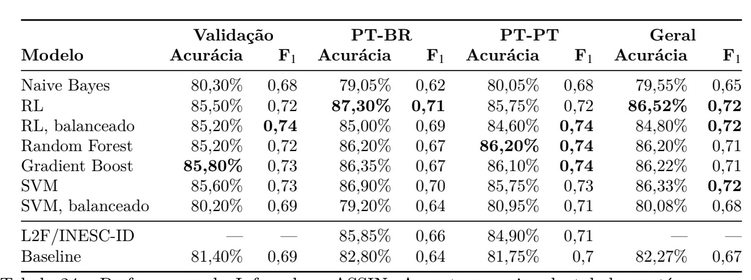
\includegraphics[width=0.7\linewidth]{Infernal-Assin}
	\caption{Resultados de modelos baseados nos features do Infernal no Assin}
	\label{fig:infernal-assin}
\end{figure}

\end{frame}

\begin{frame}[fragile]{Infernal no SICK-BR}
\begin{figure}
	\centering
	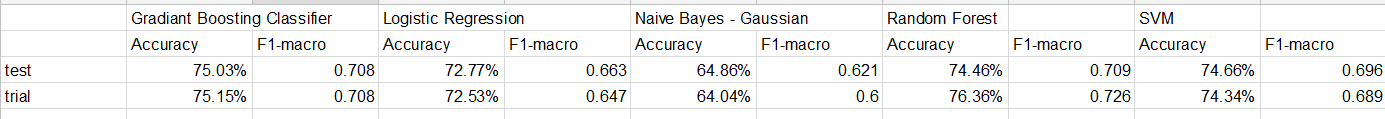
\includegraphics[width=0.7\linewidth]{Infernal-SICK-BR}
	\caption{Resultados de modelos baseados nos features do Infernal no SICK-BR}
	\label{fig:infernal-sick-br}
\end{figure}

\end{frame}


\section{Conclusões e perspectivas}
%------------------------------------------------
	\begin{frame}
\centering \textbf{Conclusões e perspectivas\\}
\end{frame}

\begin{frame}{BOW e Similaridade}
\begin{itemize}
	\item Bag of Words é um modelo com desempenho fraco.\\
	\item A similaridade é uma boa variável para a tarefa, no entanto é uma medida \textit{muito} problemática.
\end{itemize}

\end{frame}


\begin{frame}{Assin e SICK}
\begin{itemize}
	\item Os resultados foram parecidos em ambos os corpora.\\
	\item Uma questão que aparece nessas análises iniciais é a de que o SICK-BR ganharia muito se fosse maior.\\
	\item De modo geral os resultados mostram que o SICK-BR é uma ferramenta tão boa quanto o Assin para a tarefa.\\
\end{itemize}
\end{frame}


\begin{frame}{Próximos passos}
\begin{itemize}
	\item Analisar os erros e acertos do Infernal no Sick-BR\\
	\item Testar outros modelos.\\
	\item Desenvolver estratégias para aumentar o tamanho do Sick-BR de modo consistente, mantendo a qualidade do Corpus.\\
\end{itemize}
\end{frame}
\begin{frame}

\centering\large{Obrigado!}

\end{frame}

%----------------------------------------------------------------------------------------

\end{document}